\documentclass{standalone}

\usepackage{tikz}

\begin{document}


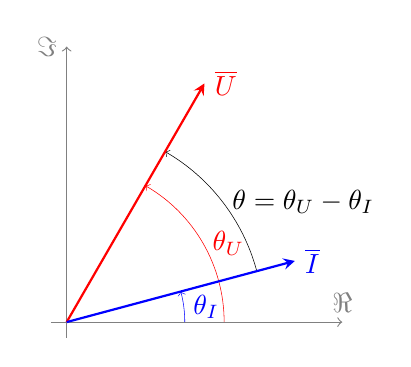
\begin{tikzpicture}
  \draw[->, thin, color=gray] (-0.2,0) -- (3.5,0) node[above] {$\Re$};
  \draw[->, thin, color=gray] (0,-0.2) -- (0,3.5) node[left] {$\Im$};
  \draw [->, very thin, color=blue](1.5,0)  arc[radius = 1.5, start angle= 0, end angle= 15] node [pos=0.5, right] {$\theta_I$};
  \draw [->, very thin, color=red](2,0)  arc[radius = 2, start angle= 0, end angle= 60] node [pos=0.5, right] {$\theta_U$};
  \draw [->, very thin, color=black](15:2.5)  arc[radius = 2.5, start angle= 15, end angle= 60] node [pos=0.5, right] {$\theta = \theta_U - \theta_I$};
  \draw[->, >=stealth, thick, color = red] (0, 0) -- (60:3.5) node[right] {$\overline{U}$};  \draw[->, >=stealth, thick, color = blue] (0, 0) -- (15:3) node[right] {$\overline{I}$};  
\end{tikzpicture}

\end{document}


